\chapter{Control Methods}\label{chap::optimization}
This section outlines the control methods used to lower the return temperature in district heating networks actuating over the bypass control valve and the supply temperature. Afterwards the application of Bayesian Optimization will be discussed. 

\section{Bypass Flow Control}
These valves are used to redirect supply water to the return network to prevent a drop in the supply water temperature during a period of low heat demand. However, the flow redirected by the bypass valve should also be limited as it increases the return temperature, therefore causing a higher overall energy loss in the network and a decrease in efficiency of the heat pump. As mentioned in Section \ref{sec::overflowmech}, the bypass valves found in the Cooltower are thermostatic bypass valves. 

Articles revolving the control of thermostatic bypasses in district heating networks are scarcely present in the literature. Even though proper control of the bypasses can play an important role in lowering the return temperature \cite{app15062982,VANDERMEULEN201845}. In \cite{VANDERMEULEN201845}, the authors propose a theoretical benchmark for the performance of bypass controllers and compare it with a thermostatic bypass valve. Where Li et al. \cite{DTUlibrary} show the impact of varying thermostatic bypass flows (installed at the branch ends) on the return temperature for different heat loads, but they do not perform an optimization. Brand et al. \cite{BRAND2014256} also investigated the effect of thermostatic bypass valves, comparing them with different bypass valve configurations linked to bathroom floor heating to improve energy efficiency. They came to the conclusion that the thermostatic bypass cannot be completely replaced by the floor heating as the flow was limited. The authors of \cite{BENAKOPOULOS2021120928} do optimize thermostatic regulation valves to achieve a better return temperature, but these are connected to the radiators on the customer site. Rong et al. \cite{RONG2025116197} created an optimization model to maximize the heat storage capacity and economic efficiency of the DHN by selectively placing bypasses and controlling the flow through these bypasses using valves. 

\section{Supply Temperature Control}
Supply temperature control maintains the network temperature at the required level by injecting or extracting the appropriate amount of heat. Traditional supply temperature control is often done via a weather compensation technique, which adjusts the supply temperature based on outdoor conditions. The weather compensation curves can vary significantly depending on the research, and in case of wrong commissioning of the curves, they can perform worse than constant supply temperatures, resulting in higher return temperatures \cite{app15062982, LIAO200555}. The adaptive control method proposed by Liao et al. \cite{LIAO200555} relies on real-time measurements of space heat load to adjust the supply temperature. It results in better meeting the heat demand. Tol et al. \cite{TOL2021105} also make use of real-time data. They present a novel demand-responsive control strategy that reacts to changes in the return supply temperature difference at substations. This doesn't necessarily lead to a lower return temperature compared to the weather compensation curves, but it reduces electricity use. The authors of \cite{papaKonstantikou} made a controller that determines the lowest supply temperature based on heat demand predictions and network time-delay calculations. 


\section{Bayesian Optimization Overview}
All the information in this section is drawn from the tutorial on Bayesian optimization written by Brochu, Cora, and de Freitas \cite{bo_tutorial}. The citations from this section are also drawn from them. 

Bayesian optimization is used to find the extrema of objective functions in cases where evaluating them is expensive. It can be applied in situations where there is no closed-form expression of the objective function, but it is possible to gather some data points of the function. Bayesian optimization techniques are highly efficient considering the number of samples needed to find an extreme. This is largely due to incorporating a prior belief about the problem into the data sampling and the balance between exploration (sampling x at high uncertainty of the objective function) and exploitation (sampling x where the objective function is likely to be high) of the search space. The technique revolves around Bayes' Theorem, stated below, hence its name. 

\begin{equation}
P(f \mid \mathcal{D}_{1:t}) \propto P(\mathcal{D}_{1:t}\mid f) P(f) .
\end{equation}
With $x_i$ as the ith sample, $f(x_i)$ as the observation of the objective function at $x_i$ and $\mathcal{D}_{1:t} = \{x_{1:t},f(x_{1:t})\}$. The prior $P(f)$ represents our belief of the space of possible objective functions. Where the posterior captures the information we have of the objective function. After every iteration, the prior of the objective function is updated with the obtained posterior of the previous iteration \todo{klopt dit?}. Bayesian optimization uses Gaussian Processes (GP) to define the prior of the function. A Gaussian Process is a distribution over Gaussian functions, completely specified by its mean function $m$ and the covariance function $k$ \cite{bo_tutorial}. 

\begin{equation}
    f(x) \sim \mathcal{GP}(m(x), k(x,x'))
\end{equation}
For convenience, the prior mean is assumed to be zero, applications in which this is not the case are, for example \cite{MartinezCantin, Brochu2010}. The covariance function is a more crucial choice for the prior, as it determines the smoothness properties of samples drawn from the GP. Depending on the type of system you want to optimize, the kernel varies. A common example of a kernel is the squared exponential kernel, Equation \ref{eq::isotropic}. With $\theta$ as a hyperparameter affecting the width of the kernel. In the case of anisotropic models, this hyperparameter becomes a diagonal matrix \cite{rasmussen2006gaussian}. It controls the influence of every feature on the covariance.
\begin{equation}\label{eq::isotropic}
k\left(\mathrm{x}_i, \mathrm{x}_j\right)=\exp \left(-\frac{1}{2 \theta^2}\left\|\mathrm{x}_i-\mathrm{x}_j\right\|^2\right),
\end{equation}
\begin{equation}\label{eq::anistropic}
k\left(\mathrm{x}_i, \mathrm{x}_j\right)=\exp \left(-\frac{1}{2}\left(\mathrm{x}_i-\mathrm{x}_j\right)^T \operatorname{diag}(\theta)^{-2}\left(\mathrm{x}-\mathrm{x}^{\prime}\right)\right).
\end{equation}
The values of the hyperparameters are usually defined by seeding with a few random samples and maximizing the log likelihood of the evidence given $\theta$ \cite{rasmussen2006gaussian, santner2003design}. The kernel choice is typically done using hierarchical Bayesian model selection \cite{mackay1992practical} or cross-validation. 

The next sample location $x_{t+1}$ is determined using an acquisition function. These functions are defined in a way that they yield high values for potentially high (or low, depending on the extreme of interest) values of the objective functions. This can be due to a high predicted value, large uncertainty, or a combination of both. Maximizing the acquisition function results in the next sample location. A proper trade-off between exploration and exploitation within this process is essential to Bayesian optimization, as it allows the method to efficiently scan the search space for potential extrema. 
Močkus et al. \cite{Mockus1978} proposed to maximize the expected improvement with respect to the best value known thus far. Lizotte \cite{Lizotte2008} introduces an extra parameter to improve the trade-off. Cox and John \cite{CoxJohn1997} present an algorithm that selects evaluation points based on the lower confidence bound of the prediction site. 

Figure \ref{fig::BO} shows three iterative steps of the Bayesian optimization technique. At each step the next sampling point is chosen based on the maximum of the acquisition function. This information is then used to update the prior, as one can clearly see as the uncertainty changes. 

\begin{figure}[h]
    \centering
    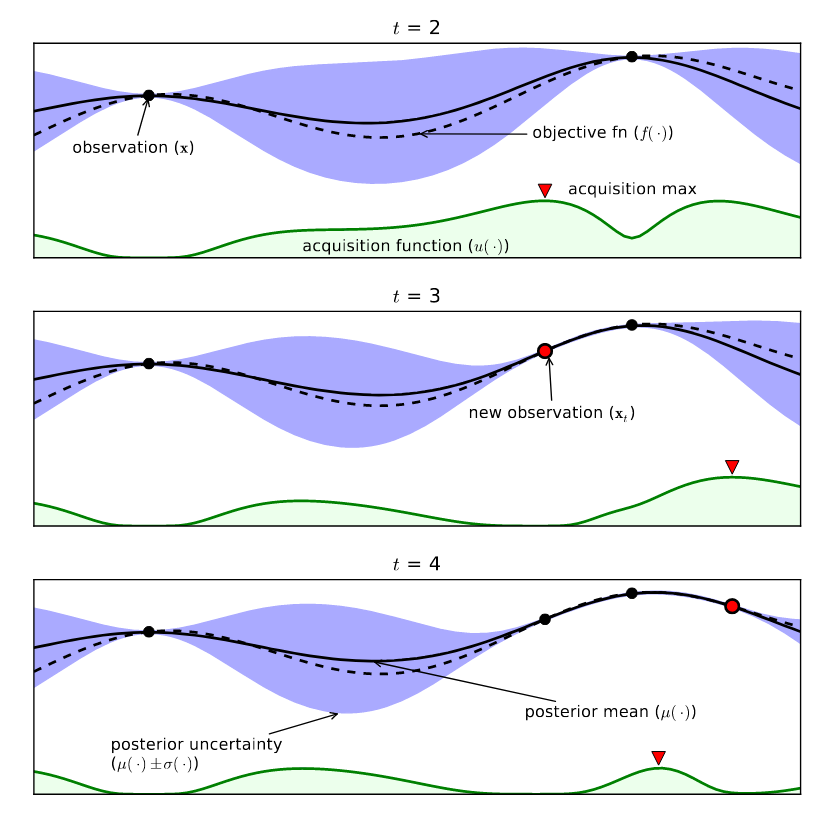
\includegraphics[width=0.6\linewidth]{Literature Survey - DCSC template/figuresLIT/BayesianOptmization.png}
    \caption{A Gaussian Process approximating the objective function of a 1D problem after four iterations using sampled values of the objective function. In this example, the sought extreme is the maximum \cite{bo_tutorial}.}
    \label{fig::BO}
\end{figure}

\section{Bayesian Optimization Application}
- paar algemene toepassingen
- kijken naar onderzoeken die zich richten op meerdere inputs

\todo[inline]{waar het wordt gebruikt voor mijn toepassing en wat voor kernel en hyperaparemeters ze daar hadden gebruikt}


\todo[inline]{dit verhaal over de mogelijke inputs en hoe dat wordt gedaan bij bayesian optimization}
Several options might be suitable to achieve both functions. A distinction can be made between passive and active control valves. The simplest passive valve would be a flow control valve that does not change its opening. The opening is found through an optimization. Another passive control would be to make use of the already present valve and optimize its temperature set point. Danfoss also supplies Pressure Indepenent Control Valves (PICV), which can guarantee a constant flow rate regardless of pressure fluctuations in the system while still maintaining the same pressure loss over the valve. Active control can also take place with the flow control valve and the PICV where the position of the valve can be remotely controlled. Creating the possibility of applying real time control.  